\documentclass{standalone}

\usepackage{tikz}\usepackage{tikz-qtree}

\usetikzlibrary{positioning,calc}

\begin{document}
	
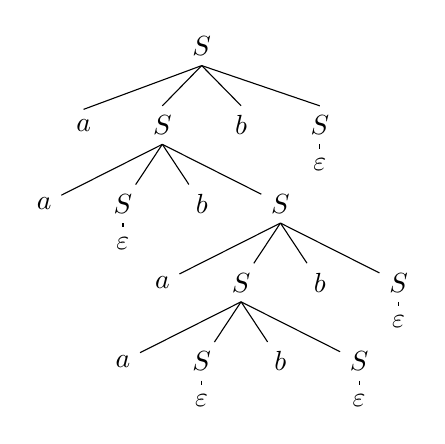
\begin{tikzpicture}
\node (root) at (0,0) {$S$};

% LEVEL 1

\node (l1n1) at ($(root)-(1.5,1)$)  {$a$};
\node (l1n2) at ($(root)-(0.5,1)$)  {$S$};
\node (l1n3) at ($(root)-(-0.5,1)$) {$b$};
\node (l1n4) at ($(root)-(-1.5,1)$) {$S$};

\draw[-] (root.south) -- (l1n1.north);
\draw[-] (root.south) -- (l1n2.north);
\draw[-] (root.south) -- (l1n3.north);
\draw[-] (root.south) -- (l1n4.north);

% LEVEL 2

\node (l2n1) at ($(l1n2)-(1.5,1)$)  {$a$};
\node (l2n2) at ($(l1n2)-(0.5,1)$)  {$S$};
\node (l2n3) at ($(l1n2)-(-0.5,1)$) {$b$};
\node (l2n4) at ($(l1n2)-(-1.5,1)$) {$S$};

\draw[-] (l1n2.south) -- (l2n1);
\draw[-] (l1n2.south) -- (l2n2);
\draw[-] (l1n2.south) -- (l2n3);
\draw[-] (l1n2.south) -- (l2n4);

% LEVEL 3

\node (l3n1) at ($(l2n4)-(1.5,1)$)  {$a$};
\node (l3n2) at ($(l2n4)-(0.5,1)$)  {$S$};
\node (l3n3) at ($(l2n4)-(-0.5,1)$) {$b$};
\node (l3n4) at ($(l2n4)-(-1.5,1)$) {$S$};

\draw[-] (l2n4.south) -- (l3n1);
\draw[-] (l2n4.south) -- (l3n2);
\draw[-] (l2n4.south) -- (l3n3);
\draw[-] (l2n4.south) -- (l3n4);

% LEVEL 4

\node (l4n1) at ($(l3n2)-(1.5,1)$)  {$a$};
\node (l4n2) at ($(l3n2)-(0.5,1)$)  {$S$};
\node (l4n3) at ($(l3n2)-(-0.5,1)$) {$b$};
\node (l4n4) at ($(l3n2)-(-1.5,1)$) {$S$};

\draw[-] (l3n2.south) -- (l4n1);
\draw[-] (l3n2.south) -- (l4n2);
\draw[-] (l3n2.south) -- (l4n3);
\draw[-] (l3n2.south) -- (l4n4);


% epsilons

\node (e1) at ($(l1n4)-(0,0.5)$) {$\varepsilon$};
\draw[-] (l1n4) -- (e1);

\node (e2) at ($(l2n2)-(0,0.5)$) {$\varepsilon$};
\draw[-] (l2n2) -- (e2);

\node (e3) at ($(l3n4)-(0,0.5)$) {$\varepsilon$};
\draw[-] (l3n4) -- (e3);

\node (e41) at ($(l4n2)-(0,0.5)$) {$\varepsilon$};
\draw[-] (l4n2) -- (e41);

\node (e42) at ($(l4n4)-(0,0.5)$) {$\varepsilon$};
\draw[-] (l4n4) -- (e42);

\end{tikzpicture}
\end{document}
